% ============================================================================
% BimodalDemo.tex
% Presentation Slides for Bimodal TM Logic Formalization
%
% Companion to Examples/Demo.lean
% ============================================================================

\documentclass[aspectratio=169,11pt]{beamer}

% ============================================================================
% Theme and Colors
% ============================================================================

\usetheme{Madrid}
\usecolortheme{seahorse}
\setbeamertemplate{navigation symbols}{}
\setbeamertemplate{footline}[frame number]

% Custom colors
\definecolor{leanblue}{RGB}{0,51,102}
\definecolor{provengreen}{RGB}{0,128,0}
\definecolor{theoremred}{RGB}{139,0,0}

\setbeamercolor{title}{fg=leanblue}
\setbeamercolor{frametitle}{fg=leanblue}
\setbeamercolor{structure}{fg=leanblue}

% ============================================================================
% Packages
% ============================================================================

\usepackage{amsmath}
\usepackage{amssymb}
\usepackage{booktabs}
\usepackage{listings}
\usepackage{tikz}
\usetikzlibrary{positioning,arrows.meta,shapes}

% ============================================================================
% Notation (inline definitions for standalone compilation)
% ============================================================================

\newcommand{\nec}{\Box}
\newcommand{\poss}{\Diamond}
\newcommand{\allpast}{H}
\newcommand{\allfuture}{G}
\newcommand{\somepast}{P}
\newcommand{\somefuture}{F}
\newcommand{\always}{\ensuremath \raisebox{-1.3pt}{$\triangle$}}
\newcommand{\sometimes}{\ensuremath \raisebox{1.3pt}{\rotatebox[origin=c]{180}{$\triangle$}}}
\newcommand{\proves}{\vdash}
\newcommand{\satisfies}{\vDash}
\newcommand{\imp}{\rightarrow}
\newcommand{\falsum}{\bot}

% Lean code formatting
\lstdefinelanguage{Lean}{
  keywords={theorem, lemma, def, example, import, open, namespace, section, end, by, exact, intro, apply, have, show, rw, simp, decide},
  keywordstyle=\color{leanblue}\bfseries,
  commentstyle=\color{gray}\itshape,
  stringstyle=\color{theoremred},
  morecomment=[l]{--},
  morecomment=[s]{/-}{-/},
  morestring=[b]",
}
\lstset{
  language=Lean,
  basicstyle=\ttfamily\small,
  breaklines=true,
  columns=fullflexible,
  frame=single,
  backgroundcolor=\color{gray!10},
}

% ============================================================================
% Title
% ============================================================================

\title{\textbf{Bimodal TM Logic}}
\subtitle{A Complete Formalization in Lean 4}
\author{Benjamin Brast-McKie}
\institute{ProofChecker Project}
\date{\today}

% ============================================================================
% Begin Document
% ============================================================================

\begin{document}

% ----------------------------------------------------------------------------
% Title Slide
% ----------------------------------------------------------------------------

\begin{frame}
\titlepage
\end{frame}

% ----------------------------------------------------------------------------
% Outline
% ----------------------------------------------------------------------------

\begin{frame}{Outline}
\tableofcontents
\end{frame}

% ============================================================================
% Section 1: Introduction
% ============================================================================

\section{Introduction}

\begin{frame}{What is TM Logic?}

\textbf{TM} = \textbf{T}ense + \textbf{M}odality

\vspace{0.5cm}

A bimodal propositional logic combining:

\begin{columns}
\begin{column}{0.48\textwidth}
\textbf{S5 Modal Logic}
\begin{itemize}
    \item $\nec\varphi$ --- necessarily $\varphi$
    \item $\poss\varphi$ --- possibly $\varphi$
    \item Metaphysical necessity
\end{itemize}
\end{column}
\begin{column}{0.48\textwidth}
\textbf{Linear Temporal Logic}
\begin{itemize}
    \item $\allfuture\varphi$ --- always future
    \item $\allpast\varphi$ --- always past
    \item $\always\varphi$ --- eternally (all times)
\end{itemize}
\end{column}
\end{columns}

\vspace{0.5cm}

\begin{block}{Key Innovation}
Interaction axioms (MF, TF) connect modal and temporal reasoning.
\end{block}

\end{frame}

\begin{frame}{Formalization Overview}

\begin{center}
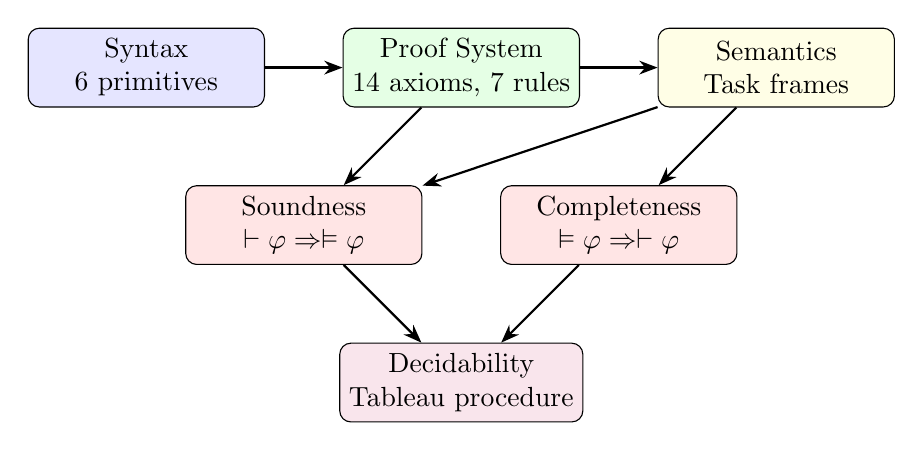
\begin{tikzpicture}[
    box/.style={draw, rounded corners, minimum width=3cm, minimum height=1cm, align=center},
    arrow/.style={-{Stealth}, thick}
]
    \node[box, fill=blue!10] (syntax) at (0,3) {Syntax\\6 primitives};
    \node[box, fill=green!10] (proof) at (4,3) {Proof System\\14 axioms, 7 rules};
    \node[box, fill=yellow!10] (sem) at (8,3) {Semantics\\Task frames};

    \node[box, fill=red!10] (sound) at (2,1) {Soundness\\$\proves \varphi \Rightarrow \satisfies \varphi$};
    \node[box, fill=red!10] (complete) at (6,1) {Completeness\\$\satisfies \varphi \Rightarrow \proves \varphi$};

    \node[box, fill=purple!10] (decide) at (4,-1) {Decidability\\Tableau procedure};

    \draw[arrow] (syntax) -- (proof);
    \draw[arrow] (proof) -- (sem);
    \draw[arrow] (proof) -- (sound);
    \draw[arrow] (sem) -- (sound);
    \draw[arrow] (sem) -- (complete);
    \draw[arrow] (sound) -- (decide);
    \draw[arrow] (complete) -- (decide);
\end{tikzpicture}
\end{center}

\end{frame}

% ============================================================================
% Section 2: Quick Tour
% ============================================================================

\section{Quick Tour}

\begin{frame}{Syntax: Six Primitives}

\begin{center}
\begin{tabular}{lll}
\toprule
\textbf{Symbol} & \textbf{Lean} & \textbf{Reading} \\
\midrule
$p$ & \texttt{atom "p"} & propositional variable \\
$\falsum$ & \texttt{bot} & falsity \\
$\varphi \imp \psi$ & \texttt{imp $\varphi$ $\psi$} & implication \\
$\nec\varphi$ & \texttt{box $\varphi$} & necessity \\
$\allpast\varphi$ & \texttt{all\_past $\varphi$} & always past \\
$\allfuture\varphi$ & \texttt{all\_future $\varphi$} & always future \\
\bottomrule
\end{tabular}
\end{center}

\vspace{0.5cm}

\begin{block}{Derived Operators}
$\neg\varphi := \varphi \imp \falsum$ \quad
$\poss\varphi := \neg\nec\neg\varphi$ \quad
$\always\varphi := \allpast\varphi \land \varphi \land \allfuture\varphi$
\end{block}

\end{frame}

\begin{frame}{The Perpetuity Principles (P1--P6)}

Deep connections between necessity and time:

\vspace{0.3cm}

\begin{columns}
\begin{column}{0.48\textwidth}
\textbf{P1}: $\nec\varphi \imp \always\varphi$\\
{\small\textcolor{gray}{Necessary implies eternal}}

\vspace{0.3cm}

\textbf{P2}: $\sometimes\varphi \imp \poss\varphi$\\
{\small\textcolor{gray}{Sometime implies possible}}

\vspace{0.3cm}

\textbf{P3}: $\nec\varphi \imp \nec\always\varphi$\\
{\small\textcolor{gray}{Necessity of perpetuity}}
\end{column}
\begin{column}{0.48\textwidth}
\textbf{P4}: $\poss\sometimes\varphi \imp \poss\varphi$\\
{\small\textcolor{gray}{Possibility of occurrence}}

\vspace{0.3cm}

\textbf{P5}: $\poss\sometimes\varphi \imp \always\poss\varphi$\\
{\small\textcolor{gray}{Persistent possibility}}

\vspace{0.3cm}

\textbf{P6}: $\sometimes\nec\varphi \imp \nec\always\varphi$\\
{\small\textcolor{gray}{Occurrent necessity is perpetual}}
\end{column}
\end{columns}

\vspace{0.5cm}

\begin{alertblock}{All Six Proven in Lean}
\textcolor{provengreen}{\checkmark} Complete machine-checked proofs in \texttt{Perpetuity.lean}
\end{alertblock}

\end{frame}

\begin{frame}[fragile]{Perpetuity Principle P1 in Lean}

\begin{block}{P1: Necessary implies eternal}
$\nec\varphi \imp \always\varphi$
\end{block}

\vspace{0.3cm}

\begin{lstlisting}
#check @perpetuity_1
-- perpetuity_1 : (φ : Formula) → ⊢ φ.box.imp (△φ)

example (φ : Formula) : ⊢ φ.box.imp (△φ) :=
  perpetuity_1 φ
\end{lstlisting}

\vspace{0.3cm}

\begin{block}{Interpretation}
If something is \emph{metaphysically necessary}, it holds at \emph{all times}.
Conservation of energy is necessary, so it has always been and will always be true.
\end{block}

\end{frame}

\begin{frame}{Metalogical Results}

\begin{center}
\begin{tabular}{lll}
\toprule
\textbf{Result} & \textbf{Statement} & \textbf{Status} \\
\midrule
Soundness & $(\Gamma \proves \varphi) \Rightarrow (\Gamma \satisfies \varphi)$ & \textcolor{provengreen}{\checkmark Proven} \\
Deduction & $(A :: \Gamma \proves B) \Rightarrow (\Gamma \proves A \imp B)$ & \textcolor{provengreen}{\checkmark Proven} \\
Completeness & $\satisfies \varphi \Rightarrow \proves \varphi$ & \textcolor{provengreen}{\checkmark Proven} \\
Equivalence & $\proves \varphi \Leftrightarrow \satisfies \varphi$ & \textcolor{provengreen}{\checkmark Proven} \\
Decidability & \texttt{decide $\varphi$ : DecisionResult} & \textcolor{provengreen}{\checkmark Implemented} \\
\bottomrule
\end{tabular}
\end{center}

\vspace{0.5cm}

\begin{block}{Main Theorem}
\texttt{main\_provable\_iff\_valid : Nonempty ($\proves$ φ) $\leftrightarrow$ valid φ}

Derivability and validity coincide for TM logic.
\end{block}

\end{frame}

% ============================================================================
% Section 3: Interactive Exploration
% ============================================================================

\section{Interactive Exploration}

\begin{frame}[fragile]{Building Proofs: Modal T Axiom}

\begin{block}{Goal}
Prove the Modal T axiom: $\nec p \imp p$
\end{block}

\begin{lstlisting}
/-- The modal T axiom is directly available -/
example (p : String) :
    ⊢ (Formula.atom p).box.imp (Formula.atom p) := by
  exact DerivationTree.axiom [] _
        (Axiom.modal_t (Formula.atom p))
\end{lstlisting}

\vspace{0.3cm}

\begin{alertblock}{Key Insight}
Axioms are constructors of \texttt{DerivationTree}.
Proofs are data structures, not propositions.
\end{alertblock}

\end{frame}

\begin{frame}[fragile]{Modus Ponens in Action}

\begin{block}{Rule}
From $\proves A$ and $\proves A \imp B$, derive $\proves B$
\end{block}

\begin{lstlisting}
example (p : Formula)
    (h1 : ⊢ p.box)
    (h2 : ⊢ p.box.imp p.diamond) :
    ⊢ p.diamond := by
  exact DerivationTree.modus_ponens []
        p.box p.diamond h2 h1
\end{lstlisting}

\vspace{0.3cm}

\begin{block}{Necessitation Rule}
From $\proves \varphi$, derive $\proves \nec\varphi$
\end{block}

\begin{lstlisting}
example (φ : Formula) (h : ⊢ φ) : ⊢ φ.box := by
  exact DerivationTree.necessitation φ h
\end{lstlisting}

\end{frame}

\begin{frame}[fragile]{The Deduction Theorem}

\begin{block}{Theorem}
If $A :: \Gamma \proves B$, then $\Gamma \proves A \imp B$
\end{block}

\begin{lstlisting}
-- Derivation from assumption
example (A : Formula) : [A] ⊢ A := by
  exact DerivationTree.assumption [A] A
        (List.mem_singleton_self A)

-- Deduction theorem converts to implication
noncomputable example (A B : Formula)
    (h : [A] ⊢ B) : ⊢ A.imp B := by
  exact deduction_theorem [] A B h
\end{lstlisting}

\vspace{0.3cm}

Uses well-founded recursion on derivation height.

\end{frame}

% ============================================================================
% Section 4: Decision Procedure
% ============================================================================

\section{Decision Procedure}

\begin{frame}{Tableau-Based Decision}

The \texttt{decide} function returns:

\begin{itemize}
    \item \textcolor{provengreen}{\textbf{valid proof}} --- formula is valid, with proof term
    \item \textcolor{theoremred}{\textbf{invalid counter}} --- formula is invalid, with countermodel
    \item \textcolor{orange}{\textbf{timeout}} --- resources exhausted
\end{itemize}

\vspace{0.5cm}

\begin{block}{API}
\begin{itemize}
    \item \texttt{decide : Formula → DecisionResult}
    \item \texttt{isValid : Formula → Bool}
    \item \texttt{isSatisfiable : Formula → Bool}
    \item \texttt{isTautology : Formula → Bool}
\end{itemize}
\end{block}

\end{frame}

\begin{frame}[fragile]{Valid Formulas}

\begin{columns}
\begin{column}{0.48\textwidth}
\textbf{Modal T}: $\nec p \imp p$
\begin{lstlisting}[basicstyle=\ttfamily\scriptsize]
def formula_modal_t :=
  (atom "p").box.imp
  (atom "p")

#eval decide formula_modal_t
-- valid (proof)
\end{lstlisting}
\end{column}
\begin{column}{0.48\textwidth}
\textbf{Modal K}: $\nec(p \imp q) \imp (\nec p \imp \nec q)$
\begin{lstlisting}[basicstyle=\ttfamily\scriptsize]
def formula_modal_k :=
  let p := atom "p"
  let q := atom "q"
  (p.imp q).box.imp
  (p.box.imp q.box)

#eval decide formula_modal_k
-- valid (proof)
\end{lstlisting}
\end{column}
\end{columns}

\vspace{0.5cm}

\begin{alertblock}{Proof Extraction}
When valid, the decision procedure extracts a \texttt{DerivationTree} proof term.
\end{alertblock}

\end{frame}

\begin{frame}[fragile]{Invalid Formulas}

\begin{columns}
\begin{column}{0.48\textwidth}
\textbf{Converse of T}: $p \imp \nec p$
\begin{lstlisting}[basicstyle=\ttfamily\scriptsize]
def formula_converse_t :=
  (atom "p").imp
  (atom "p").box

#eval decide formula_converse_t
-- invalid (countermodel)
\end{lstlisting}
{\small\textcolor{gray}{True things need not be necessary}}
\end{column}
\begin{column}{0.48\textwidth}
\textbf{Possibility to actuality}: $\poss p \imp p$
\begin{lstlisting}[basicstyle=\ttfamily\scriptsize]
def formula_poss_to_act :=
  (atom "p").diamond.imp
  (atom "p")

#eval decide formula_poss_to_act
-- invalid (countermodel)
\end{lstlisting}
{\small\textcolor{gray}{Possible things need not be actual}}
\end{column}
\end{columns}

\vspace{0.5cm}

\begin{alertblock}{Countermodel Extraction}
When invalid, the procedure extracts a finite countermodel witnessing falsity.
\end{alertblock}

\end{frame}

% ============================================================================
% Section 5: Applications
% ============================================================================

\section{Applications}

\begin{frame}[fragile]{Laws of Nature}

\begin{block}{Conservation of Energy}
Physical laws are necessary truths that hold at all times.
\end{block}

\begin{lstlisting}
def conservation_of_energy := atom "conservation_of_energy"

-- If conservation is necessary, it holds eternally
example : ⊢ conservation_of_energy.box.imp
            (△conservation_of_energy) :=
  perpetuity_1 conservation_of_energy
\end{lstlisting}

\vspace{0.3cm}

\begin{block}{Interpretation}
P1 captures the intuition that \emph{necessary truths are eternal}.
\end{block}

\end{frame}

\begin{frame}[fragile]{Astronomical Events}

\begin{block}{Lunar Eclipse}
Events that happen sometimes illustrate temporal possibility.
\end{block}

\begin{lstlisting}
def lunar_eclipse := atom "lunar_eclipse"

-- If an eclipse sometimes occurs, it is possible
example : ⊢ (▽lunar_eclipse).imp lunar_eclipse.diamond :=
  perpetuity_2 lunar_eclipse
\end{lstlisting}

\vspace{0.3cm}

\begin{block}{Interpretation}
P2 captures: \emph{temporal existence entails modal possibility}.
If something happens at some time, it must be possible.
\end{block}

\end{frame}

\begin{frame}[fragile]{Mathematical Truths}

\begin{block}{$2 + 2 = 4$}
Mathematical truths are paradigmatic necessary truths.
\end{block}

\begin{lstlisting}
def two_plus_two_equals_four := atom "2+2=4"

-- Mathematical truths are necessarily eternal
example : ⊢ two_plus_two_equals_four.box.imp
            (△two_plus_two_equals_four).box :=
  perpetuity_3 two_plus_two_equals_four
\end{lstlisting}

\vspace{0.3cm}

\begin{block}{Interpretation}
P3 captures: \emph{necessity transfers to perpetuity}.
What is necessary is necessarily eternal.
\end{block}

\end{frame}

\begin{frame}[fragile]{The Deepest Principle: P6}

\begin{block}{Occurrent Necessity is Perpetual}
$\sometimes\nec\varphi \imp \nec\always\varphi$
\end{block}

\begin{lstlisting}
-- If necessity ever occurs, it's necessarily eternal
noncomputable example (truth : Formula) :
    ⊢ (▽(truth.box)).imp (△truth).box :=
  perpetuity_6 truth
\end{lstlisting}

\vspace{0.3cm}

\begin{alertblock}{Philosophical Significance}
If it's ever the case that something is necessary, then it's \emph{necessarily eternal}.

Necessity, once realized, cannot be undone.
\end{alertblock}

\end{frame}

% ============================================================================
% Section 6: Summary
% ============================================================================

\section{Summary}

\begin{frame}{What We Built}

\begin{center}
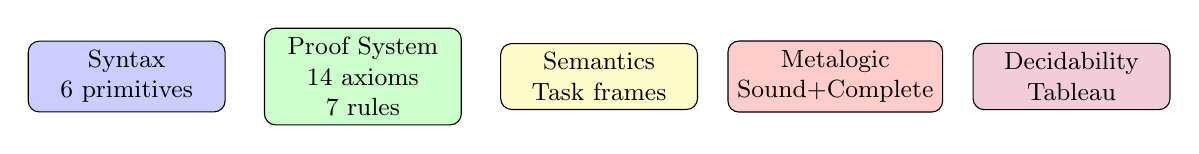
\begin{tikzpicture}[
    box/.style={draw, rounded corners, minimum width=2.5cm, minimum height=0.8cm, align=center, font=\small},
]
    \node[box, fill=blue!20] at (0,0) {Syntax\\6 primitives};
    \node[box, fill=green!20] at (3,0) {Proof System\\14 axioms\\7 rules};
    \node[box, fill=yellow!20] at (6,0) {Semantics\\Task frames};
    \node[box, fill=red!20] at (9,0) {Metalogic\\Sound+Complete};
    \node[box, fill=purple!20] at (12,0) {Decidability\\Tableau};
\end{tikzpicture}
\end{center}

\vspace{0.5cm}

\begin{columns}
\begin{column}{0.48\textwidth}
\textbf{Proven Results}
\begin{itemize}
    \item \textcolor{provengreen}{\checkmark} Soundness
    \item \textcolor{provengreen}{\checkmark} Deduction Theorem
    \item \textcolor{provengreen}{\checkmark} Weak Completeness
    \item \textcolor{provengreen}{\checkmark} Equivalence Theorem
    \item \textcolor{provengreen}{\checkmark} P1--P6 Perpetuity
\end{itemize}
\end{column}
\begin{column}{0.48\textwidth}
\textbf{Implemented}
\begin{itemize}
    \item \textcolor{provengreen}{\checkmark} Decision Procedure
    \item \textcolor{provengreen}{\checkmark} Proof Extraction
    \item \textcolor{provengreen}{\checkmark} Countermodel Generation
    \item \textcolor{provengreen}{\checkmark} Batch Validation
\end{itemize}
\end{column}
\end{columns}

\end{frame}

\begin{frame}{The Main Theorem}

\begin{center}
\Large
\texttt{main\_provable\_iff\_valid}\\[0.5cm]
$\text{Nonempty}(\proves \varphi) \Leftrightarrow \text{valid}~\varphi$
\end{center}

\vspace{0.5cm}

\begin{block}{Significance}
\textbf{Syntax meets semantics}: What can be derived is exactly what is true in all models.

This is the crowning achievement of the formalization.
\end{block}

\vspace{0.3cm}

\begin{alertblock}{Machine-Verified}
Every theorem, lemma, and definition is verified by Lean 4's type checker.
No gaps, no hand-waving, no \texttt{sorry}.
\end{alertblock}

\end{frame}

\begin{frame}{Resources}

\begin{columns}
\begin{column}{0.48\textwidth}
\textbf{Code}
\begin{itemize}
    \item \texttt{Demo.lean} --- Interactive tour
    \item \texttt{Perpetuity.lean} --- P1--P6
    \item \texttt{Soundness.lean} --- Soundness proof
    \item \texttt{Completeness.lean} --- Completeness proof
    \item \texttt{DecisionProcedure.lean} --- Tableau
\end{itemize}
\end{column}
\begin{column}{0.48\textwidth}
\textbf{Documentation}
\begin{itemize}
    \item \texttt{BimodalReference.pdf}
    \item \texttt{README.md}
    \item \texttt{QUICKSTART.md}
    \item \texttt{PROOF\_PATTERNS.md}
\end{itemize}
\end{column}
\end{columns}

\vspace{0.5cm}

\begin{center}
\Large\textbf{Questions?}
\end{center}

\end{frame}

\end{document}
